% !TeX encoding = UTF-8
% !TeX spellcheck = ca_ES
\documentclass[CAT,BIB]{TFUOC}%IB: CASTELLÀ, CAT: CATALÀ, ENG: ANGLÈS

%Begin Carles customization{

    %Load packages
        %Modifies ToC: include References, remove LoF, LoT
        \usepackage[nottoc, notlof, notlot, numbib]{tocbibind}

%        %Insert page number in reference
%        \usepackage{varioref}

        %Convert references into links
        \usepackage{hyperref}
        \hypersetup{
            colorlinks=true,
            allcolors=darkblueUOC,
            pdfauthor=Carles Criado Ninà,
        }

        %Use acronyms
        \usepackage[acronym,nomain,section=section,numberedsection=autolabel]{glossaries}
            % Make glossary links black
            \renewcommand*{\glstextformat}[1]{\textcolor{black}{#1}}
            % Generate the glossary
            \makeglossaries
            % Define acronyms:
            \newacronym{tfm}{TFM}{treball de final de màster}
            \newacronym{cq}{CQ}{qualitat de \textit{clustering} (\textit{clustering quality})}
            \newacronym{ae}{AE}{\textit{autoencoder}}
            \newacronym{fl}{FL}{aprenentatge de característiques \textit{(feature learning)}}
            \newacronym{rl}{RL}{capa de representació \textit{(representation layer)}}
            \newacronym{lf}{LF}{característiques apreses \textit{(learned features)}}
            \newacronym{mlp}{MLP}{\textit{multilayer perceptron}}
            \newacronym{cnn}{CNN}{\textit{convolutional neural network}}
            \newacronym{dbn}{DBN}{\textit{deep belief network}}
            \newacronym{gan}{GAN}{\textit{generative adversarial network}}
            \newacronym{lstm}{LSTM}{\textit{long short-term memory}}
            \newacronym{cae}{CAE}{\textit{convolutional autoencoder}}
            \newacronym{vae}{VAE}{\textit{variational autoencoder}}
            \newacronym{lstmae}{LSTM-AE}{\textit{long short-term memory autoencoder}}
            \newacronym{aae}{AAE}{\textit{adversarial autoencoder}}
            \newacronym{dae}{DAE}{\textit{denoising autoencoder}}
            \newacronym{sae}{SAE}{\textit{stacked autoencoder}}
            \newacronym{elbo}{ELBO}{límit inferior de la evidència (\textit{evidenve lower bound})}
            \newacronym{kl}{KL}{Kullback-Leibler}

        %Insert names of references with \cref{}
        \usepackage[catalan,noabbrev,nameinlink]{cleveref}
            %Use with catalan language: replace "gràfic" with "figura":
            \crefname{figure}{figura}{figures}
            \Crefname{figure}{Figura}{Figures}

        %Use \citet{} to citate inline, or \citep{} to reference between brackets
        \usepackage[square,numbers,sort&compress]{natbib}

        %Use to insert text boxes. Example:
        %    \begin{tcolorbox}[title=Títol, colback=red!5!white, colframe=red!50!black]
        %        Contingut...
        %    \end{tcolorbox}
        \usepackage{tikz, tcolorbox}
        \newcommand{\todo}[1]{
            \begin{tcolorbox}[title=ToDo!, colback=red!5!white, colframe=red!50!black, coltext=red!50!black]
            #1
            \end{tcolorbox}}

        %Provides \mathbb{}, necessary for some maths symbols
        \usepackage{amsfonts}

        %Use small font for image captions
        \usepackage[font=footnotesize,labelfont=bf]{caption}

%        %Insert sideways figure
%        \usepackage{rotating}

%        %Insert landscape page
%        \usepackage{lscape}





    %Force all nested enumerate lists to be numbered
    \renewcommand{\labelenumii}{\arabic{enumi}.\arabic{enumii}}
    \renewcommand{\labelenumiii}{\arabic{enumi}.\arabic{enumii}.\arabic{enumiii}}
    \renewcommand{\labelenumiv}{\arabic{enumi}.\arabic{enumii}.\arabic{enumiii}.\arabic{enumiv}}

%}End Carles customization

%Introducció de dades del treball
\title{Desenvolupament d'un model de \textit{deep clustering} en dades metabolòmiques utilitzant un \textit{Variational Autoencoder}}
\titcrt{VAE-DC en dades metabolòmiques} %Títol curt que apareixerà a la capçalera
\author{Carles Criado Ninà}
\date{30 de febrer de 2099}


\nomPDC{Esteban Vegas Lozano}
\nomPRA{Carles Ventura Royo}
\titulac{Màster en Bioinformàtica i Bioestadística}
\area{Àrea 3}
\idioma{Català}
\credits{15}
\parcla{clustering, deep learning, variational autoencoder, metabolomics}

\licenc{ccBy}
%Possibles llicències
%ccByNcNd
%ccByNcSa
%ccByNc
%ccByNd
%ccBySa
%ccBy
%GNU
%copyright


%%%%%%%%%%
% Resum en l'idioma

\abstractidioma{
Màxim 250 paraules, amb la finalitat, context d’aplicació, metodologia, resultats i conclusions del treball.
}

% Resum en anglès.
\abstractenglish{
A maximum of 250 words, detailing the purpose, context of application, methodology, results and conclusions of the work.
}

\begin{document}

\estructura

\tableofcontents

\listoffigures

\listoftables




\chapter{Introducció}
    %Aquesta plantilla es concep com una guia per a l’estudiant. Es pot adaptar a les necessitats de cada treball, sempre que el/la tutor/a del treball hi estigui d’acord.

    \section{Context i justificació del treball}
        %Punt de partida del treball (Quina és la necessitat a cobrir? Per què és un tema rellevant? Com es resol el problema de moment?) i aportació realitzada (Quin resultat es vol obtenir?).
        %
        %És important tenir en compte que el treball final ha de ser comprensible per a qualsevol persona que conegui l'àrea de coneixement, però no té perquè ser experta en el tema del que versa el treball.

        Una de les problemàtiques característiques del camp de la bioinformàtica és que les dades que s'estudien habitualment contenen un nombre molt elevat de variables, però un nombre reduït de mostres. Aquesta elevada dimensionalitat de les dades suposa una dificultat a l'hora de realitzar estudis estadístics.

        Un dels conjunts de tècniques estadístiques utilitzades en dades bioinformàtiques són els estudis de \textit{clustering}. Aquestes tècniques es basen en agrupar les dades en funció de la seva similitud i permeten extreure informació del conjunt de les dades, com per exemple la seva estructura latent \citep{Karim2021, Masood2015}.

        Les tècniques de \textit{clustering} clàssiques no funcionen bé en dades amb una elevada dimensionalitat, i això suposa una limitació en l'estudi de dades bioinformàtiques. Una solució alternativa que s'utilitza habitualment per combatre aquest problema és la d'aplicar primer una tècnica de reducció de la dimensionalitat, com per exemple l'anàlisi de components principals, i aplicar posteriorment les tècniques de \textit{clustering} sobre les dades transformades \citep{Min2018, Masood2015}.

        Un dels avantatges de les xarxes neuronals és que admeten treballar amb dades amb una dimensionalitat elevada. Això ha fet possible desenvolupar un gran nombre de mètodes de \textit{clustering} basats en \textit{deep learning}, que es poden dividir en dos grans grups: mètodes basats reduir la dimensionalitat i aplicar mètodes de \textit{clustering} sobre les dades transformades; i mètodes que desenvolupen un model de \textit{clustering} sobre les dades originals sense transformar \citep{Karim2021}.

        En aquest estudi es pretén desenvolupar un model de \textit{deep clustering} basat en l'arquitectura \textit{Variational Autoencoder}, un tipus de model generatiu que es basa en mètodes probabilístics Bayesians \citep{Kingma2019}. El model resultant s'aplicarà sobre un conjunt de dades metabolòmiques obtingut d'un anàlisi clínic i es valorarà la interpretabilitat del resultat en funció de la relació entre els clústers generats i els grups clínics diferenciats en l'estudi.

    \section{Objectius del treball}
    \label{s:objectius}
        %Llistat dels objectius del treball.

        \begin{enumerate}
            \item Desenvolupar un mètode de \textit{deep clustering} basat un model de \textit{Variational autoencoder}, aplicat a un conjunt de dades metabolòmiques.
            \begin{enumerate}
                \item Contextualitzar el problema a resoldre realitzant una extensiva recerca bibliogràfica.
                \item Desenvolupar un model de \textit{deep clustering} utilitzant un \textit{variational autoencoder}.
                \item Aplicar el model desenvolupat a un conjunt de dades metabolòmiques i estudiar els resultats.
            \end{enumerate}
        \end{enumerate}

    \section{Impacte en sostenibilitat, ètic-social i de diversitat}
    \label{s:etic}
        %Aquesta secció hauria d'identificar els impactes positius i/o negatius del treball final en les tres dimensions de la competència transversal UOC “Compromís ètic i global”.
        %La Guia transversal sobre la Competència Ètica i Global us ajudarà a redactar aquests apartats.


    \section{Enfocament i mètode seguit}
        %Menció de quines són les possibles estratègies per dur a terme el treball i quina és l’estratègia triada (desenvolupar un producte nou, adaptar un producte existent…). Cal incloure una valoració de per què aquesta és l’estratègia més apropiada per aconseguir els objectius.


    \section{Planificació del treball}
        %Descripció dels recursos necessaris per fer el treball, les tasques a realitzar i una planificació temporal de cada tasca mitjançant un diagrama de Gantt o similar. Aquesta planificació hauria de marcar quins són les fites parcials de cadascuna de les PAC.

        \subsection{Tasques:}
        \label{sec:tasques}

            A continuació es llisten les tasques a realitzar per la consecució dels objectius definits a la \cref{sec:objectius_especifics}. Al diagrama de Gantt de la \cref{fig:gantt} es reflecteix el temps assignat a cada tasca.

            \begin{enumerate}
                \item %Objectiu 1
                \begin{enumerate}
                    \item Caracteritzar les tècniques clàssiques de \textit{clustering} aplicades a dades metabolòmiques.
                    \item Caracteritzar les tècniques de \textit{clustering} basades en \textit{deep learning}.
                    \item Estudiar en profunditat l’arquitectura de \textit{variational autoencoder} i com s’aplica en \textit{clustering}.
                    \item Estudiar el funcionament de Keras, practicar utilitzant exemples.
                \end{enumerate}

                \item %Objectiu 2
                \begin{enumerate}
                    \item Obtenir un conjunt de dades adequat per a realitzar l'estudi.
                    \item Realitzant un estudi preliminar amb tècniques clàssiques que servirà com a marc de referència.
                    \item Desenvolupar un model de \textit{deep clustering}.
                    \item Comparar els resultats obtinguts amb el marc de referència.
                \end{enumerate}

                \item %Objectiu 3
                \begin{enumerate}
                    \item Aplicar el model a un conjunt de dades metabolòmiques.
                    \item Estudiar la interpretabilitat dels resultats comparant els clústers generats amb els grups reals de les dades.
                \end{enumerate}
            \end{enumerate}

        \subsection{Calendari:}
        \label{sec:calendari}

            A la \cref{fig:gantt} es mostra un diagrama de Gantt on es representa el temps assignat a cada tasca, així com a altres activitats relacionades amb el TFM com són la redacció dels informes de les diferents PACs, l'elaboració de la memòria i de la presentació i la preparació de la defensa.

            En la planificació s'ha tingut en compte el pla docent i els dies festius. S'ha calculat una dedicació de 4 hores per dia laborable, encara que s'ha contemplat la possibilitat de dedicar temps addicional puntualment per assegurar el compliment de les fites. En total, es preveu una dedicació de 312 hores.

            \begin{figure}[htpb]
                \centering
                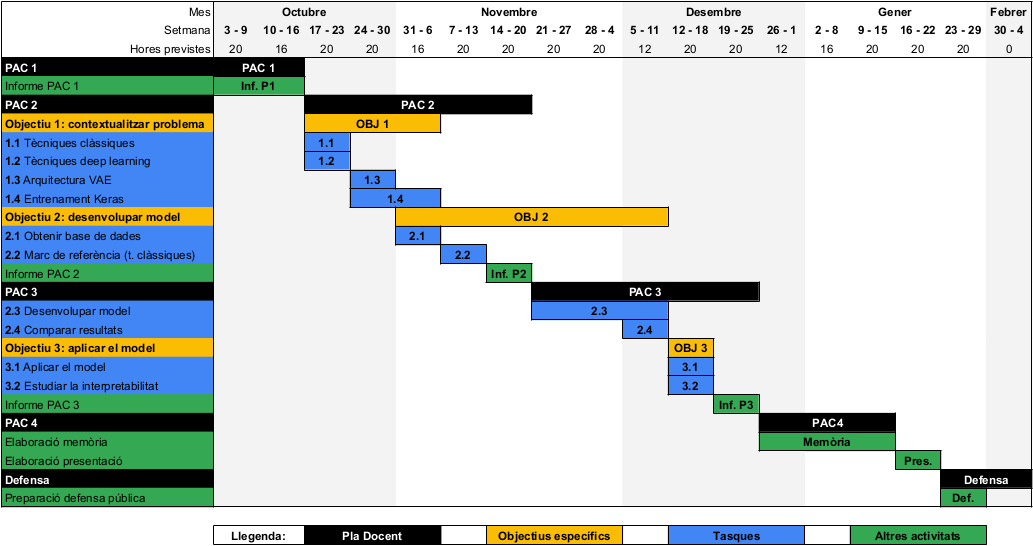
\includegraphics[width=\textwidth]{TFM_calendari.png}
                \caption{Diagrama de Gantt.}
                \label{fig:gantt}
            \end{figure}

        \subsection{Fites:}
        \label{sec:fites}

            S'han definit les següents fites com a dates clau per planificar el treball:

            \begin{description}
                \item[17/10/2022] Elaboració del pla de treball. Entrega de l'informe de la PAC 1.
                \item[28/10/2022] Finalitzar la recerca bibliogràfica (marc teòric).
                \item[04/11/2022] Data límit per a l'obtenció d'un conjunt de dades.
                Consecució de l'objectiu 1.
                \item[21/11/2022] Entrega de l'informe de la PAC 2.
                \item[09/12/2022] Consecució de l'objectiu 2.
                \item[16/12/2022] Consecució de l'objectiu 3.
                \item[24/12/2022] Entrega de l'informe de la PAC 3.
                \item[15/01/2023] Entrega de la memòria.
                \item[23/01/2023] Presentació i defensa preparades.
            \end{description}


    \section{Breu sumari de productes obtinguts}
        %No cal entrar en detall: la descripció detallada es farà a la resta de capítols.

    \section{Breu descripció dels altres capítols de la memòria}
        %Breu explicació dels continguts de cada capítol i la seva relació amb el projecte global.

\chapter{Estat de l'art}
\label{s:state}
    %Estat de l'art del tema en qüestió.
    %Hauria d'acabar mostrant per què el treball és important i aporta alguna cosa, i amb les hipòtesis del treball.

\todo{Falta incorporar moltes referències, sobretot a les \cref{s:state_reduccio,s:state_ae}.}

    \section{Metabolòmica}
    \label{s:state_metabol}

\todo{
    Pendent de definir el tipus de dades que treballarem. En principi esperem que siguin dades metabolòmiques. En aquest secció farem un molt breu resum (2-3 paràgrafs) de la tècnica i el tipus de dades obtingudes. Finalitzarem mencionant l'objectiu d'aplicar \textit{clustering}, per connectar-ho amb la següent secció.
}

    \section{Tècniques de \textit{clustering}}
    \label{s:state_cluster}

        Les tècniques de \textit{clustering} són un conjunt de tècniques d'aprenentatge automàtic no supervisat que es basen en agrupar les dades en funció d'alguna mesura de la seva similitud, sense coneixement previ de l'estructura de les dades o el nombre de grups que es pretén obtenir.

        L'objectiu d'aquestes tècniques és separar les dades en diversos grups que siguin internament homogenis (els objectes dins el mateix grup són similars entre ells) i tinguin característiques diferents a la resta de grups.

        Identificar aquests grups permet obtenir informació sobre l'estructura de les dades com la presència de patrons, i pot servir com a un punt de partida en l'exploració de les dades. Per exemple, aplicades a dades metabolòmiques, les tècniques de \textit{clustering} poden permetre identificar diferents tipus cel·lulars en funció de la seva expressió metabòlica \citep{Blekherman2011}.

        Existeix una gran varietat de tècniques de \textit{clustering} \citep{Karim2021, Min2018, Blekherman2011, Masood2015}. Encara que totes comparteixen un mateix objectiu, aborden el problema aplicant diferents criteris i per tant els grups que formen poden no coincidir. Algunes de les aproximacions més utilitzades històricament es basen en mètodes matemàtics i estadístics \citep{Masood2015}, com mètodes jeràrquics, mètodes basats en centroides, distribucions o densitats \citep{Karim2021}.

        \textbf{Mètodes jeràrquics:} es basen en crear clústers amb un ordre predeterminat, on els clústers de més baix nivell es combinen iterativament per crear clústers més grans. Això els dota d'una estructura jeràrquica que es pot presentar en forma de dendrograma, però implica que l'assignació de cada punt a un clúster és determinista. Aquests algoritmes són sensibles al soroll \citep{Karim2021}.

        \textbf{Mètodes basats en centroides:} (p. ex. \textit{k-means}) es basen assignar cada punt a un número predeterminat de grups i calcular els seus centroides. Després es canvia iterativament l'assignació de cada punt als diferents grups fins a minimitzar la suma de les distàncies de cada punt al centroide del seu grup. En general aconsegueixen un millor rendiment que els mètodes jeràrquics, però son incapaços de trobar grups no convexos \citep{Karim2021}.

        \textbf{Mètodes basats en distribucions:} (p. ex. model de barreja gaussiana (GMM)) es basen en modelar els grups en funció d'una barreja de distribucions probabilístiques. La seva base estadística permet inferir relacions entre les característiques de les dades, però requereix de fortes assumpcions sobre la distribució de les dades i tenen tendència a sobre-ajustament \citep{Karim2021}.

        \textbf{Mètodes basats en densitats:} (p. ex. DBSCAN) defineixen els clústers com àrees amb major densitat comparats amb la resta de les dades. Els punts en regions més disperses es consideren fronteres o soroll. El punt negatiu d'aquests mètodes és precisament que requereixen d'una disminució de la densitat per detectar les fronteres dels clústers i són poc eficaces en separar grups contigus \citep{Karim2021}.

    \section{Reducció de la dimensionalitat}
    \label{s:state_reduccio}

        Un dels problemes que apareix habitualment al analitzar dades bioinformàtiques és la seva elevada dimensionalitat, característica que fa que les tècniques de \textit{clustering} clàssiques no funcionin bé \citep{Masood2015, Karim2021}. Per combatre aquest problema, una solució és aplicar tècniques de reducció de la dimensionalitat i posteriorment aplicar les tècniques de \textit{clustering} sobre les dades transformades \citep{Min2018, Masood2015}.

        La reducció de la dimensionalitat s'aconsegueix mitjançant tècniques d'\gls{fl}. L'objectiu d'aquestes tècniques és representar les dades originals en un espai dimensional inferior, aplicant una transformació que retingui el màxim d'informació. L'espai reduït resultant s'anomena \gls{rl} i les seves dimensions \gls{lf}.

        Històricament s'han utilitzat tècniques matemàtiques per realitzar \gls{fl}, que poden ser transformacions lineals (anàlisi de components principals) o no lineals (mètodes kernel o tècniques espectrals). Posteriorment s'apliquen les tècniques de clustering sobre les \gls{lf}.

        Una limitació dels mètodes lineals és que no són capaços de retenir informació sobre relacions no lineals en les dades, el que provoca una reducció de la \gls{cq}. Les tècniques no lineals són més adequades \citep{Karim2021}.

    \section{Tècniques de \textit{deep clustering}}
    \label{s:state_deep}

        Les xarxes neuronals profundes possibiliten aplicar tècniques de \gls{fl} més eficients que les descrites a la secció anterior, aplicant mètodes no lineals complexes que permeten capturar \gls{lf} més rellevants. En particular, la funció de transformació es pot optimitzar mitjançant l'aprenentatge dels paràmetres de la xarxa, el que permet extreure \gls{lf} òptimes per obtenir una bona \gls{cq} \citep{Karim2021}.

        La seva recent popularització ha fet possible desenvolupar un gran nombre de tècniques de \textit{clustering} basades en \textit{deep learning}, anomenades en conjunt tècniques de \textit{deep clustering}. Es poden dividir en dos grans grups: mètodes de dos passos, que es basen en utilitzar tècniques de \gls{fl} i aplicar mètodes de \textit{clustering} convencionals sobre les \gls{lf}; i mètodes d'un sol pas que desenvolupen un model de \textit{clustering} sobre les dades originals \citep{Karim2021}.

        A la literatura s'ha descrit una gran varietat de mètodes basats en diferents arquitectures neuronals (\gls{mlp}, \gls{cnn}, \gls{dbn}, \gls{gan}, \gls{ae}). A \url{https://github.com/rezacsedu/Deep-learning-for-clustering-in-bioinformatics} \citep{Karim2021} es pot trobar un llistat amb enllaços als articles originals.

        La majoria d'aproximacions actuals utilitzen una arquitectura basada en un \gls{ae} \citep{Karim2021}, donat que és capaç d'obtenir \gls{lf} eficients per realitzar \textit{clustering}.


    \section{\textit{Autoencoder}}
    \label{s:state_ae}

        L'arquitectura \gls{ae} està formada per dues parts: un codificador i un descodificador. La funció del codificador és representar l'entrada en un espai dimensional reduït, sovint un vector, anomenat codi. La funció del descodificador és reconstruir l'entrada original a partir del codi.

        Optimitzant els paràmetres d'ambdues parts conjuntament durant l'entrenament de la xarxa es busca aconseguir que el codificador sigui capaç de comprimir la entrada mantenint el màxim d'informació. Aplicant la idea de \gls{fl}, el codi esdevé la \gls{rl}.

        Per aconseguir un \textit{clustering} eficaç, no és suficient amb aquesta optimització ja que si no s'aplica cap restricció a la \gls{rl} podria donar lloc a \gls{lf} que no permeten una bona \gls{cq}. Per resoldre aquest problema es defineixen dos tipus de funció de cost, que s'optimitzen conjuntament durant l'entrenament \citep{Min2018}:
        \begin{itemize}
            \item La \textbf{funció de cost auxiliar}, que depèn de la capacitat del codificador d'obtenir una \gls{rl} eficient que permeti que el descodificador sigui capaç de regenerar l'entrada. Garanteix obtenir \gls{lf} rellevants.
            \item La \textbf{funció de cost de \textit{clustering}}, que depèn de l'algoritme de \textit{clustering} i de que les \gls{lf} obtingudes siguin adequades per realitzar \textit{clustering}. Assegura obtenir una bona \gls{cq}.
        \end{itemize}

        L'aproximació més bàsica de l'arquitectura \gls{ae} es pot construir utilitzant \glspl{mlp} simètrics pel codificador i descodificador. Encara que és fàcil d'implementar, el model generat conté un gran nombre d'hiperparàmetres i esdevé difícil d'optimitzar i balancejar les dues funcions de cost \citep{Karim2021}. A més, no s'aplica cap restricció a la funció de representació i per tant no garanteix obtenir una bona \gls{cq}.

        A la literatura s'han descrit diferents aproximacions a la idea del \gls{ae}, que prenen com a base altres arquitectures. Algunes d'aquestes aproximacions permeten aconseguir un model generatiu, que és capaç de generar dades similars a les d'entrenament. Alguns d'aquestes aproximacions són:

        \textbf{\Gls{cae}:} l'arquitectura \gls{ae} estàndard no dona bons resultats per trobar patrons en imatges (dades amb invariança espacial). Per combatre-ho, es poden combinar amb \gls{cnn} utilitzant convolucions al codificador del \gls{ae} (i les corresponents desconvolucions al descodificador), on els filtres de la \gls{cnn} són un paràmetre que es pot optimitzar (en lloc de construir-los a mà com en una \gls{cnn} estàndard).

        \textbf{\Gls{vae}:} aquesta aproximació es basa en mètodes Bayesians, el que li atorga certa robustesa estadística que no tenen altres arquitectures. Es tracten les dades com a mostres d'una distribució desconeguda i s'aplica una restricció al codificador perquè les representi com una barreja de distribucions conegudes (per exemple, gaussianes). Els paràmetres que aprèn la xarxa són els paràmetres de les distribucions (mitjana i variància). El descodificador reconstrueix les mostres originals, el que permet generar mostres aleatòries semblants a la distribució original desconeguda. S'explica amb més detall a la \cref{s:metodes_vae}.

        \textbf{\Gls{lstmae}:} de manera similar al cas del \gls{cae}, l'arquitectura \gls{ae} estàndard no funciona bé amb dades seqüencials, però es pot combinar amb l'arquitectura \gls{lstm}. El codificador es forma combinant capes \gls{lstm}, on la última capa codifica un vector que representa l'entrada de la xarxa. El descodificador, també format per capes \gls{lstm}, pren aquest vector (replicat per adaptar-lo a l'entrada de la primera capa \gls{lstm}) i reconstrueix l'entrada original.

        \textbf{\Gls{aae}:} aquesta aproximació pren la idea del discriminador de la arquitectura \gls{gan} i la introdueix al \gls{ae}. L'objectiu és representar les dades originals com una barreja de distribucions conegudes, de manera similar al \gls{vae}. En aquest cas la xarxa està formada per tres parts: el codificador, que redueix l'entrada a un codi, el descodificador, que reconstrueix la entrada a partir del codi, i un discriminador. El discriminador intenta discriminar entre els codis generats i punts mostrejats aleatòriament de la distribució escollida. El resultat és que els codis generats acaben aproximant-se a aquesta distribució \citep{Makhzani2015}.

        \textbf{\Gls{dae}:} aquesta tècnica entrena el \gls{ae} introduint soroll a l'entrada del codificador i reconstruint les dades originals amb el descodificador. Això permet aprendre una representació més robusta de les dades i també la reconstrucció de les dades originals a partir d'unes dades parcialment corrompudes.

        \textbf{\Gls{sae}:} diversos \gls{ae} es poden apilar per aconseguir representacions més comprimides de les dades d'entrada. S'entrena un primer \gls{ae} per comprimir i reconstruir les dades d'entrada i es pren el codi comprimit. Aquest codi es pren com l'entrada d'un segon \gls{ae}, que s'entrena per comprimir i reconstruir el codi. Aquest procés es repeteix fins a aconseguir el nombre de capes desitjat. Finalment, s'ordenen les capes codificadores i descodificadores de cada \gls{ae} seqüencialment, formant un \gls{sae}, i s'entrena una última vegada el model sencer per ajustar tots els pesos. D'aquesta manera s'obté un model capaç de codificar les dades en un espai dimensional més reduït.

        En aquest \gls{tfm}, es desenvoluparà un model de \textit{deep clustering} utilitzant una arquitectura \gls{vae}, ja que les seves característiques el fan un model interessant. El model probabilístic li atorga certa robustesa estadística que pot ser útil al extreure conclusions del resultats obtinguts. Alhora, la capacitat generativa pot permetre generar mostres artificials semblants a les originals, el que podria servir com a tècnica d'augment de dades (\textit{data augmentation}).


\chapter{Materials i mètodes}
    %En aquests apartats, cal descriure:
    %\begin{itemize}
    %    \item Els aspectes més rellevant del disseny i desenvolupament del treball.
    %    \item La metodologia triada per a fer aquest desenvolupament, descrivint les alternatives possibles, les decisions preses, i els criteris utilitzats per prendre aquestes decisions.
    %    \item Els productes obtinguts.
    %\end{itemize}
    %\textbf{L’estructuració dels capítols pot variar segons el tipus de treball.}

    \section{Model de \textit{deep clustering}}
    \label{s:metodes_dc}

    En aquest \gls{tfm}
    es pretén implementar un model de \textit{deep clustering} en dades metabòliques.
    Com s'ha descrit a les \cref{s:state_deep,s:state_ae},
    existeix una gran varietat d'arquitectures de xarxes neuronals descrites a la literatura.
    Intentar estudiar totes les possibilitats seria inabastable donat el temps disponible,
    pel que ha sigut necessari acotar l'estudi a una única arquitectura.
    S'ha decidit implementar una aproximació basada en \gls{vae},
    donat que presenta algunes característiques interessants.

    Com s'ha mencionat a la \cref{s:state_ae},
    l'arquitectura \gls{vae} és una implementació específica de \gls{ae}
    basada en mètodes Bayesians.
    Això li atorga al model certa robustesa estadística
    que no trobem en altres arquitectures.
    A més,
    la \gls{rl} apresa permet la generació de mostres artificials
    similars a les dades d'entrenament.
    Això últim pot resultar útil com a tècnica d'augment de dades.

    \subsection{Variational Autoencoder}
    \label{s:metodes_vae}

        A continuació es fa una breu presentació del model \gls{vae},
        basada en les referències \citep{Kingma2014,Kingma2019}.
        No s'entrarà en profunditat en les explicacions matemàtiques.
        Per una explicació més detallada es recomana llegir les fonts originals.

        En l'arquitectura \gls{ae},
        el codificador aprèn una representació de l'entrada $\mathbf{x}$
        en un espai dimensional reduït $\mathbf{z}$
        aplicant una transformació no lineal.
        Des de la perspectiva de \gls{fl},
        aquest espai reduït es correspon amb la \gls{rl}.
        El descodificador aprèn a reconstruir $\mathbf{x}$ a partir de $\mathbf{z}$
        aplicant una segona transformació no lineal.
        L'entrenament de les dues parts conjuntament
        aconsegueix que les \gls{lf} siguin una bona representació de les dades originals.

        En l'aproximació que pren el \gls{vae},
        s'assumeix que l'entrada $\mathbf{x}$ és un conjunt d'observacions de variables aleatòries,
        que provenen d'un procés desconegut
        amb una distribució $p^*(\mathbf{x})$.
        Aquesta distribució és desconeguda,
        de manera que intentem aproximar-la amb un model $p_\theta(\mathbf{x})$,
        on $\theta$ són els paràmetres del model.

        L'espai $\mathbf{z}$ es considera un conjunt de variables latents del model
        que segueixen una distribució $p_\theta(\mathbf{z})$.
        Les variables latents són variables que estan presents al model però no observem en les dades.
        Es pot fixar que $p_\theta(\mathbf{z})$ sigui una distribució fàcil de computar,
        per exemple una barreja de gaussianes.

        Sota aquesta premissa,
        el model a inferir és sobre una distribució conjunta $p_\theta(\mathbf{x,z})$
        de les variables observades i latents.
        L'objectiu del codificador és aprendre els paràmetres $\theta$
        de la distribució $p_\theta(\mathbf{z|x})$
        (la distribució posterior de $\mathbf{z}$ condicionada a $\mathbf{x}$)
        De la mateixa manera,
        l'objectiu del descodificador és aprendre els paràmetres $\theta$
        de la distribució $p_\theta(\mathbf{x|z})$.
        A la \cref{fig:vae_kingma} s'il·lustra
        com el model relaciona els espais $\mathbf{x}$ i $\mathbf{z}$.

        \begin{figure}
            \centering
            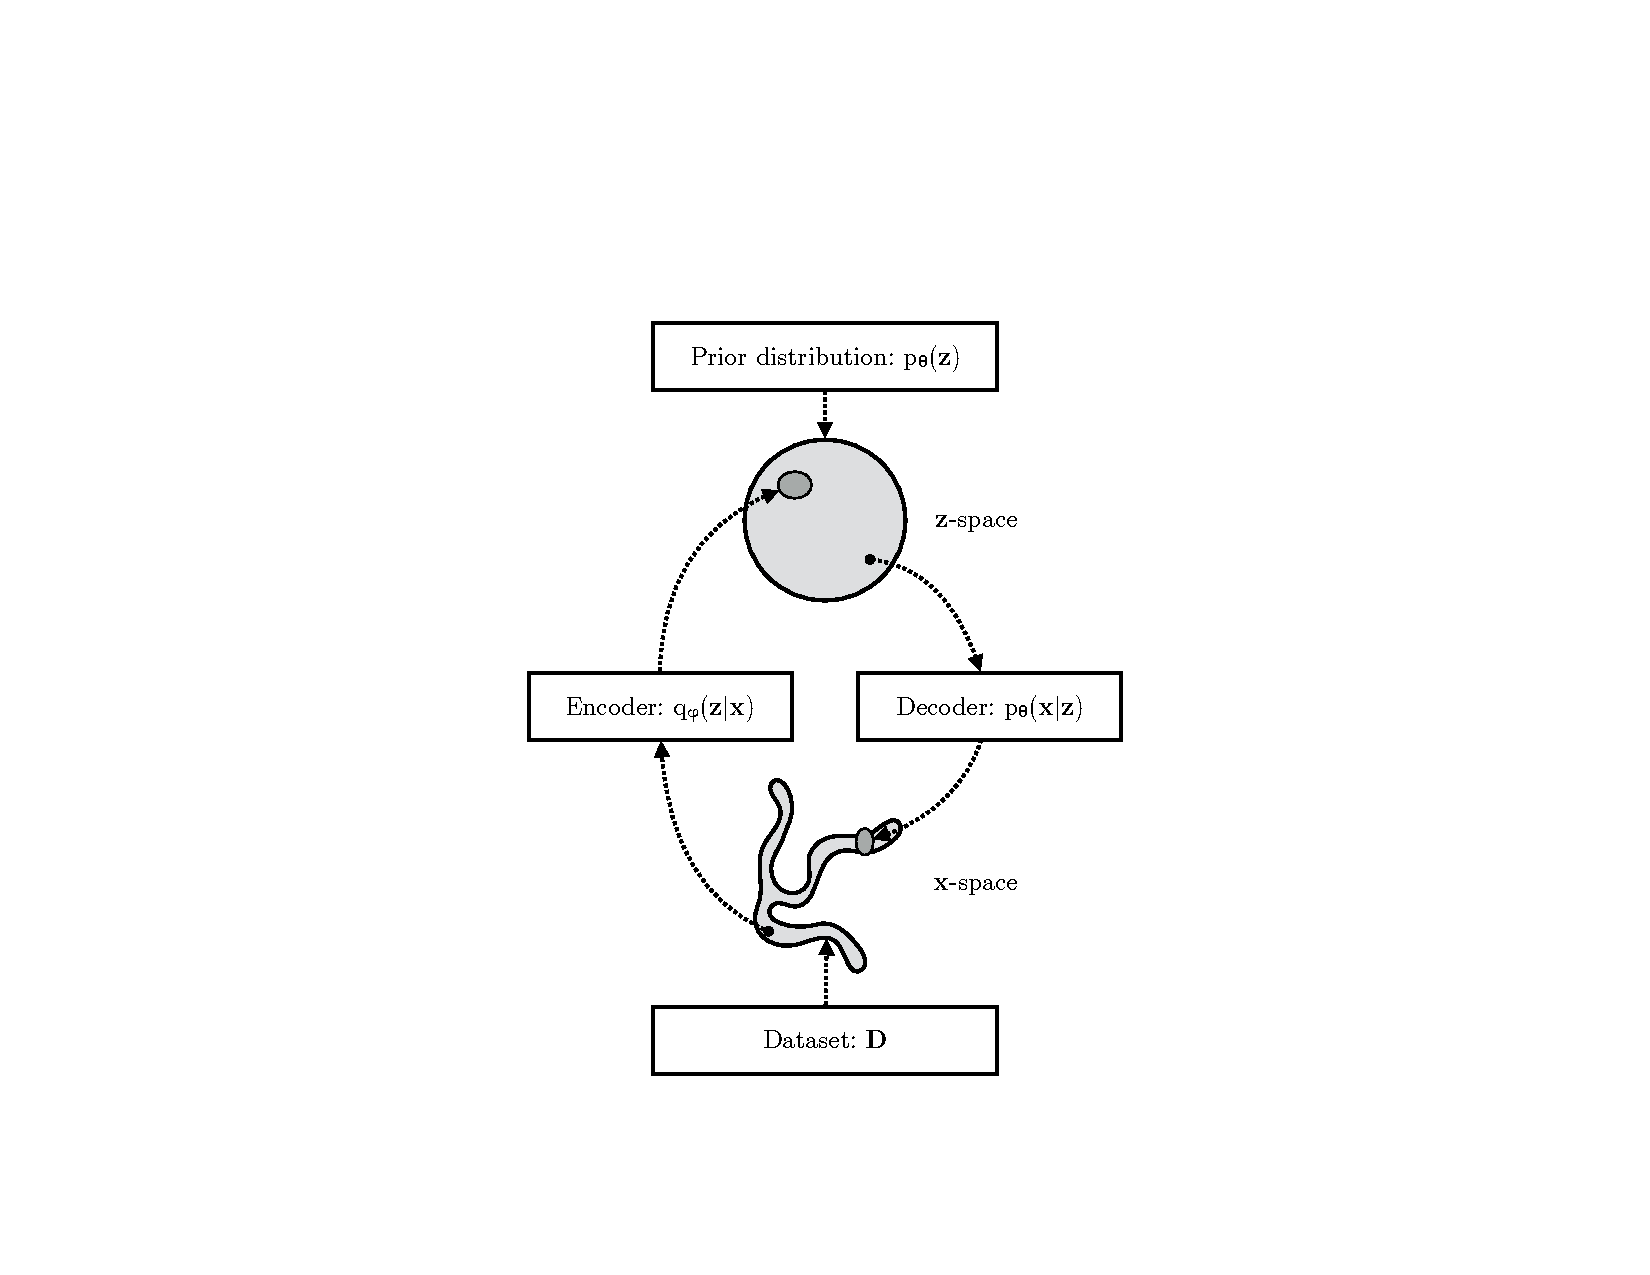
\includegraphics[width=0.5\textwidth]{kingma2019_vae.pdf}
            \caption{
                Esquema del model \gls{vae}.
                Les dades observades $\mathbf{D}$ (\textit{dataset})
                són una mostra d'unes variables de l'espai $\mathbf{x}$,
                que segueix una distribució intractable.
                L'espai latent $\mathbf{z}$ s'escull que segueixi
                una distribució $p_\phi(\mathbf{z})$ fàcil de computar.
                El codificador (\textit{encoder})
                troba la distribució condicional de $\mathbf{z}$ donada $\mathbf{x}$,
                aconseguint una representació de les mostres a l'espai latent.
                El decodificador (\textit{decoder})
                troba la distribució condicional de $\mathbf{x}$ donada $\mathbf{z}$,
                aconseguint la reconstrucció de les dades a partir de l'espai latent.
                Font: Kingma and Welling, 2019 \citep{Kingma2019}
            }
            \label{fig:vae_kingma}
        \end{figure}

    \subsection{Optimització dels paràmetres}
    \label{s:vae_optimitzacio}

        El codificador pretén aprendre els paràmetres $\theta$ òptims
        de la distribució $p_\theta(\mathbf{z|x})$,
        que està condicionada per la distribució marginal $p_\theta(\mathbf{x})$
        segons la equació:
        \begin{equation}
        \label{eq:cond_p_z_on_x}
            p_\theta(\mathbf{z|x}) =
            \frac {p_\theta(\mathbf{x,z})}
                  {p_\theta(\mathbf{x})}
        \end{equation}

        Aquesta distribució marginal en el model bé donada per:
        \begin{equation}
        \label{eq:marginal_p_x}
            p_\phi(\mathbf{x}) = \int p_\phi(\mathbf{x, z}) d\mathbf{z}
        \end{equation}

        La integral en la \cref{eq:marginal_p_x} provoca que
        la distribució marginal $p_\theta(\mathbf{x})$ no tingui un estimador eficient
        i sigui intractable computacionalment.
        Això provoca que no es pugui diferenciar respecte als paràmetres $\theta$
        i optimitzar-la pel mètode del descens de gradients.
        En conseqüència,
        tampoc es poden optimitzar els paràmetres de la distribució $p_\theta(\mathbf{z|x})$.

        En el seu lloc,
        es pot inferir un model $q_\phi(\mathbf{z|x})$
        que aproximi la distribució intractable $p_\theta(\mathbf{z|x})$,
        on els paràmetres $\phi$ s'aprenen a través de la optimització
        dels pesos i biaixos de la xarxa neuronal.

        La diferència entre aquestes dues distribucions
        es pot calcular mitjançant la divergència de \gls{kl}:
        $D_{KL} ( q_\phi(\mathbf{z|x}) \| p_\theta(\mathbf{z|x}) )$.
        L'objectiu és minimitzar aquesta divergència,
        però no és possible calcular-la directament
        donada la intractabilitat de $p_\theta(\mathbf{z|x})$.

        Aquesta divergència es relaciona amb la distribució marginal
        segons la següent igualtat:

        \begin{equation}
            \label{eq:kl}
            \log p_\theta(\mathbf{x}) =
            \mathcal{L}_{\theta,\phi}(\mathbf{x}) +
            D_{KL} (
            q_\phi(\mathbf{z|x}) \|
            p_\theta(\mathbf{z|x})
            )
        \end{equation}

        Per tant, es pot minimitzar la divergència maximitzant el terme $\mathcal{L}_{\theta,\phi}(\mathbf{x})$.
        Aquest terme s'anomena \gls{elbo}
        ja que la divergència \gls{kl} és sempre no negativa i
        per tant \gls{elbo} és el límit inferior de $\log p_\theta(\mathbf{x})$
        (evidència de $\mathbf{x}$):

        \begin{equation}
            \label{eq:lim_inf}
            \log p_\theta(\mathbf{x}) \ge
            \mathcal{L}_{\theta,\phi}(\mathbf{x})
        \end{equation}

        El terme \gls{elbo} es calcula segons la següent equació:

        \begin{equation}
        \label{eq:elbo}
            \mathcal{L}_{\theta,\phi}(\mathbf{x}) =
            \mathbb{E}_{q_\phi(\mathbf{z|x})}
                [ \log p_\theta(\mathbf{x|z}) ] -
            \mathbb{E}_{q_\phi(\mathbf{z|x})} \left[
                \log \frac {q_\phi(\mathbf{z|x})}
                           {p_\theta(\mathbf{z})}
            \right]
        \end{equation}

        La maximització del \gls{elbo} implica:
        \begin{itemize}
            \item Maximitzar el primer terme de la equació,
            la esperança de $\log p_\theta(\mathbf{x|z})$,
            que es correspon amb optimitzar els paràmetres del descodificador.
            És a dir, s'aconsegueix una millor reconstrucció.

            \item Minimitzar el segon terme,
            la esperança de $\log ( q_\phi(\mathbf{z|x}) / p_\theta(\mathbf{z}) )$,
            que és la divergència \gls{kl} entre
            la distribució inferida pel codificador $q_\phi(\mathbf{z|x})$
            i la distribució $p_\theta(\mathbf{z})$ fixada de l'espai latent.
            És a dir, s'aconsegueix millorar la representació obtinguda pel codificador.
        \end{itemize}

    \subsection{Descens de gradients}
    \label{s:vae_gradients}

        Per optimitzar els paràmetres de la xarxa neuronal
        de tal manera que es maximitzi el \gls{elbo},
        s'utilitza el descens de gradients.
        Per tant, cal calcular els gradients del \gls{elbo}
        amb respecte als paràmetres $\theta$ i $\phi$.

        El \gls{elbo} es pot reformular de la següent manera,
        el que facilitarà el càlcul dels gradients:

        \begin{equation}
        \label{eq:elbo_2}
            \mathcal{L}_{\theta,\phi}(\mathbf{x}) =
            \mathbb{E}_{q_\phi(\mathbf{z|x})} [
                \log p_\theta(\mathbf{x,z}) -
                \log q_\phi(\mathbf{z|x})
            ]
        \end{equation}

        I els gradients es calculen segons:

        \begin{equation}
        \label{eq:gradient_theta}
            \nabla_\theta \mathcal{L}_{\theta,\phi}(\mathbf{x}) =
            \nabla_\theta \mathbb{E}_{q_\phi(\mathbf{z|x})} [
            \log p_\theta(\mathbf{x,z}) -
            \log q_\phi(\mathbf{z|x})
            ]
        \end{equation}
        \begin{equation}
        \label{eq:gradient_phi}
            \nabla_\phi \mathcal{L}_{\theta,\phi}(\mathbf{x}) =
            \nabla_\phi \mathbb{E}_{q_\phi(\mathbf{z|x})} [
            \log p_\theta(\mathbf{x,z}) -
            \log q_\phi(\mathbf{z|x})
            ]
        \end{equation}

        Per la regla de la integral de Leibniz, el gradient en la \cref{eq:gradient_theta} es pot moure a dins de la esperança i això permet la seva computació. Però el mateix no és possible en la \cref{eq:gradient_phi}, ja que l'esperança està en funció de $\phi$.

        Per resoldre aquest problema es planteja la següent solució:
        reparametritzar la variable $\mathbf{z} \sim q_\theta(\mathbf{z|x})$
        com una funció d'una altra variable aleatòria $\epsilon$, donades $\mathbf{x}$ i $\phi$:

        \begin{equation}
        \label{eq:epsilon}
            \epsilon \sim p(\epsilon)
        \end{equation}
        \begin{equation}
        \label{eq:z_reparam}
            \mathbf{z} = g(\phi, \mathbf{x}, \epsilon)
        \end{equation}

        On la funció $g(\cdot)$ és una transformació determinista.
        Aquesta reparametrització s'il·lustra a la \cref{fig:reparametritzacio}.
        Llavors, el \gls{elbo} es pot reescriure
        en funció de $\mathbb{E}_{p_(\epsilon)}$
        en lloc de $\mathbb{E}_{q_\phi(\mathbf{z|x})}$,
        de manera que ``s'externalitza'' la aleatorietat de la variable $\mathbf{z}$
        a la nova variable $\epsilon$.
        La nova forma del gradient del \gls{elbo} en respecte a $\phi$ és:

        \begin{equation}
        \label{eq:gradient_phi_reparam}
            \nabla_\phi \mathcal{L}_{\theta,\phi}(\mathbf{x}) =
            \nabla_\phi \mathbb{E}_{p(\epsilon)} [
                \log p_\theta(\mathbf{x,z}) -
                \log q_\phi(\mathbf{z|x})
            ]
        \end{equation}

        Després d'aquesta reparametrització,
        es poden calcular els gradients del \gls{elbo}
        respecte als paràmetres $\phi$ i $\theta$,
        i així optimitzar-los mitjançant el descens de gradients.

        \begin{figure}
            \centering
            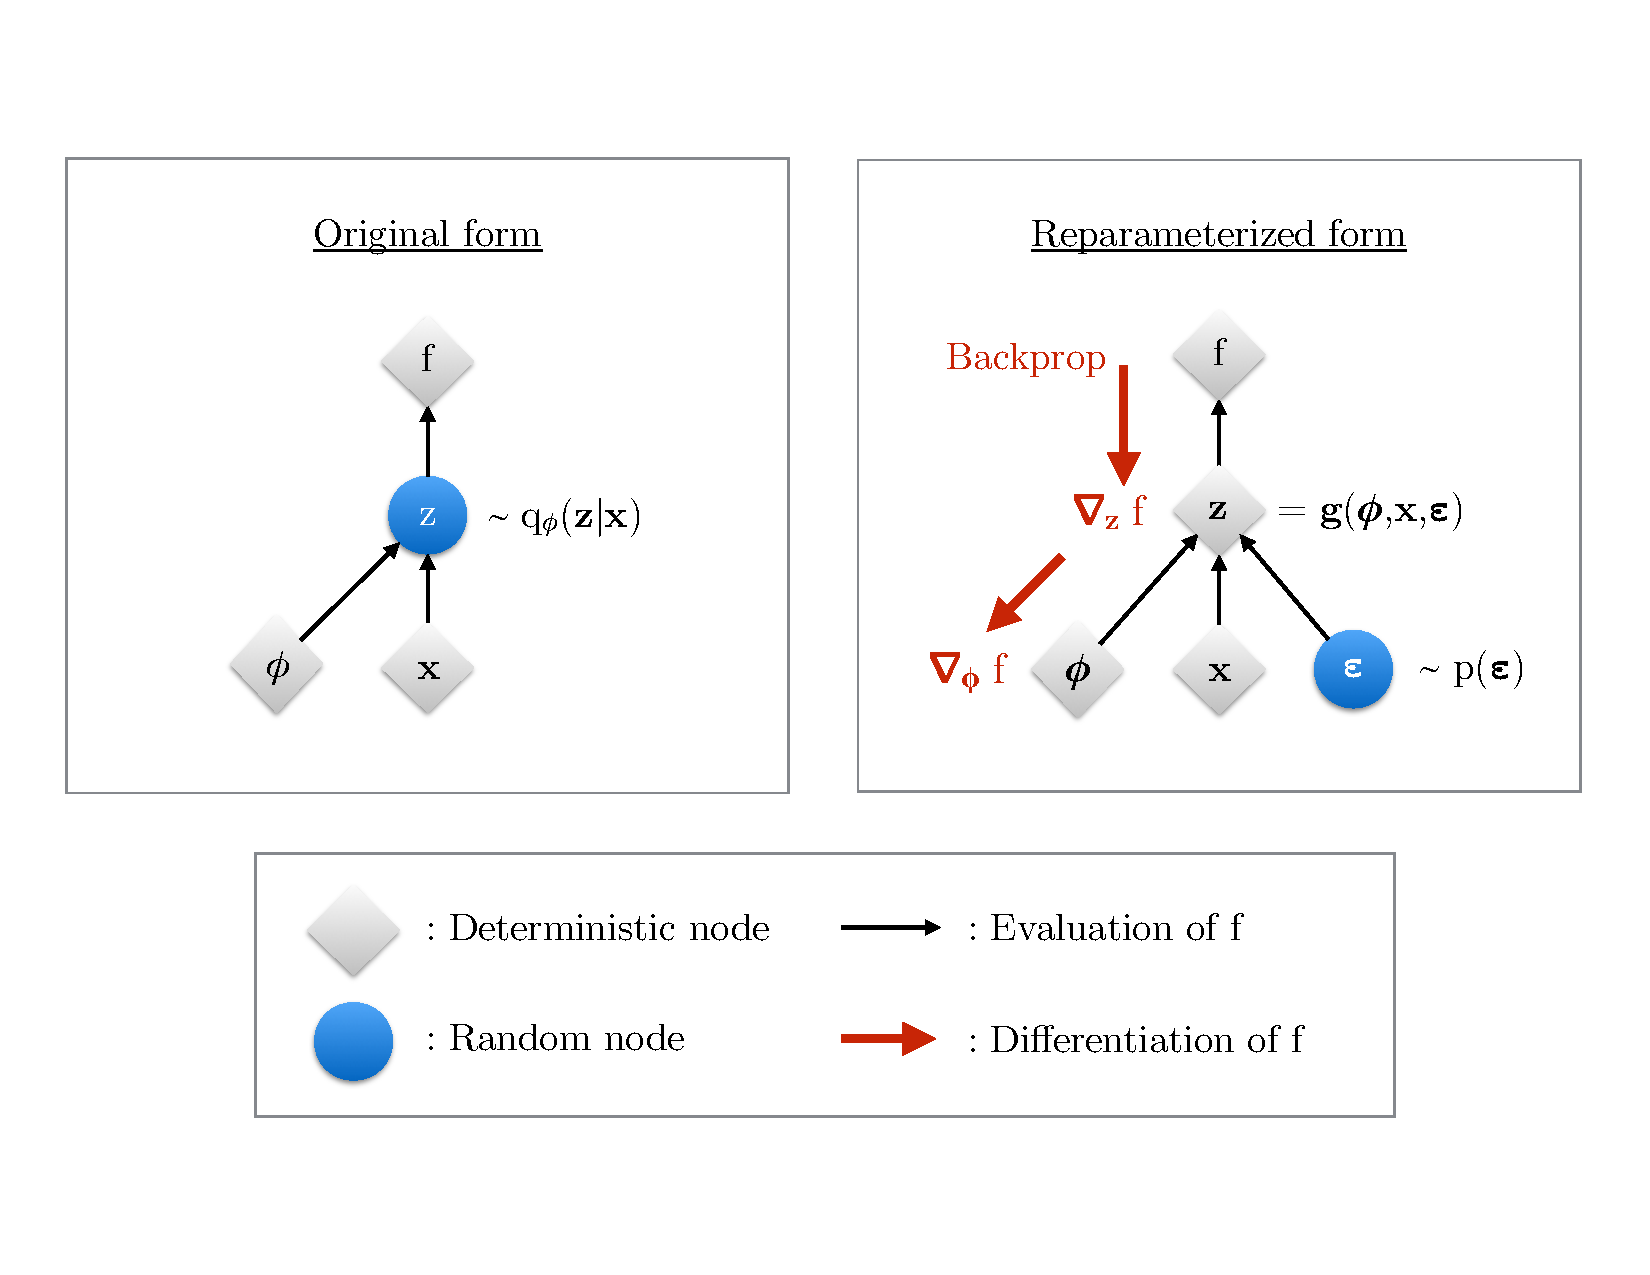
\includegraphics[width=0.7\textwidth]{kingma2019_reparam.pdf}
            \caption{
                Il·lustració de la reparametrització de $\mathbf{z}$.
                Per optimitzar els paràmetres $\theta$
                es necessita calcular els gradients de la funció d'optimització $f$
                amb respecte a $\theta$.
                En la figura de l'esquerra (forma original)
                no es pot diferenciar $f$ amb respecte a $\theta$
                perquè no es poden propagar endarrere els gradients
                a través de la variable aleatoria $\mathbf{z}$.
                Després de la reparametrització (figura de la dreta),
                la aleatorietat queda ``externalitzada'' a la variable $\epsilon$,
                i $\mathbf{z}$ depèn d'una funció $g(\cdot)$ determinista.
                Aquesta configuració sí permet propagar endarrere els gradients.
                Font: Kingma and Welling, 2019 \citep{Kingma2019}
            }
            \label{fig:reparametritzacio}
        \end{figure}

    \subsection{Implementació del model}
    \label{s:vae_implementacio}

        Un cop presentada la base teòrica,
        a continuació es resumeix com s'ha implementat el model \gls{vae}
        que s'ha construït en aquest \gls{tfm}.
        S'ha escollit que la variable latent $\mathbf{z}$
        segueixi una distribució barreja de gaussianes:

        $$\mathbf{z} \sim \mathcal{N}(\mu, \sigma^2)$$

        On $\mu$ és el vector de mitjanes de les distribucions
        i $\sigma^2$ és la matriu de variàncies.
        Per simplificar els càlculs s'ha escollit una matriu diagonal,
        de mode que $\sigma^2$ es pot escriure com un vector.

        Així, el codificador i el descodificador del \gls{vae} són
        dues xarxes neuronals amb paràmetres $\theta$ i $\phi$, respectivament.
        Aquests paràmetres són l'arquitectura de la xarxa neuronal,
        juntament amb els pesos pesos i biaixos de cada neurona.

        El codificador pren com entrada els valors de les variables observades,
        en forma d'un vector $\mathbf{x}$ per cada observació,
        i té com a sortida dos vectors:
        un vector $\mu$ amb les mitjanes de la barreja de gaussianes,
        i un vector $\sigma^2$ amb les corresponents variàncies
        (codificades com a $\log \sigma^2$ per motius de computació).

        El descodificador pren com entrada un punt de l'espai latent $\mathbf{z}$
        i té com a sortida un vector amb la mateixa forma que $\mathbf{x}$.

        En l'arquitectura \gls{ae},
        durant la fase d'entrenament
        es connecta la sortida del codificador a l'entrada del descodificador.
        Així, les dues xarxes s'entrenen conjuntament
        utilitzant el descens de gradient estocàstic.
        En el caso de l'arquitectura \gls{vae},
        és necessari aplicar la reparametrització
        explicada en la \cref{s:vae_gradients}.
        Un cop aplicada, es pot reescriure $\mathbf{z}$ com:

        $$\epsilon \sim \mathcal{N}(0, \mathbf{I})$$
        $$\mathbf{z} = \mu + \sigma \odot \epsilon$$

        On $\odot$ és el producte per elements.

        En la implementació del \gls{vae},
        s'insereix una capa neuronal sense pesos o biaixos
        enter el codificador i el descodificador.
        Aquesta capa pren com entrada la sortida del codificador
        (vectors $\mu$ i $\sigma^2$),
        obté una mostra aleatòria de la distribució de $\epsilon$
        i calcula un valor de $\mathbf{z}$,
        que passa a l'entrada del descodificador.
        A la \cref{fig:vae_kingma} es mostren esquemàticament
        les diferents parts del \gls{vae}.

        Per entrenar la xarxa neuronal en conjunt,
        s'han definit dues funcions de cost
        (il·lustrades a la \cref{fig:vae_losses})
        que corresponen als dos termes del \gls{elbo},
        segons la \cref{eq:elbo}.

        \begin{itemize}
            \item \textbf{Funció de cost de la reconstrucció:}
            computa la diferència entre l'entrada del codificador
            i la sortida del descodificador
            (la reconstrucció de l'entrada).
            Minimitzant-la, es maximitza el terme
            $\mathbb{E}_{q_\phi(\mathbf{z|x})} [ \log p_\theta(\mathbf{x|z}) ]$
            del \gls{elbo}.

            \item \textbf{Funció de cost de regularització:}
            computa la distància \gls{kl}
            entre la distribució de $\mathbf{z} \sim \mathcal{N}(\mu, \sigma^2)$
            i una distribució $\mathcal{N}(0, \mathbf{I})$.
            Minimitzant-la, es minimitza el terme
            $\mathbb{E}_{q_\phi(\mathbf{z|x})} [ \log ( q_\phi(\mathbf{z|x}) / p_\theta(\mathbf{z}) ) ]$
            del \gls{elbo}.
            S'anomena així ja que actua com a regularitzador
            de la sortida del codificador,
            assegurant que l'espai latent segueixi la distribució desitjada.
        \end{itemize}

        \begin{figure}
            \centering
            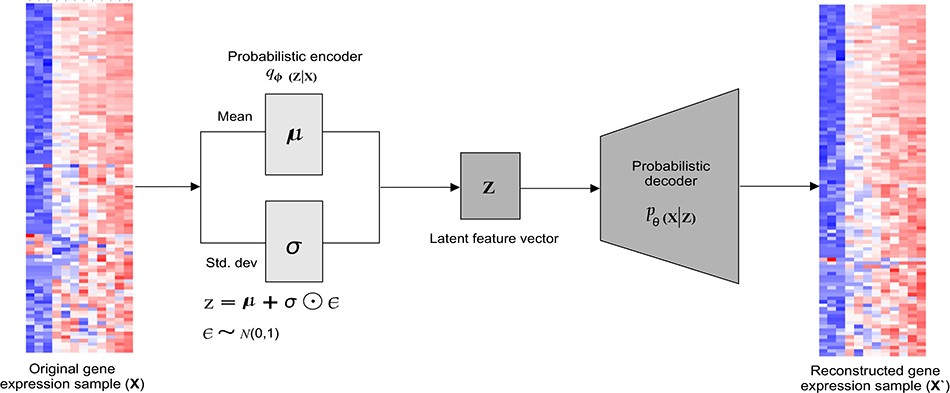
\includegraphics[width=\textwidth]{karim2021_vae.jpeg}
            \caption{
                Representació esquemàtica d'una arquitectura \gls{vae}.
                El codificador aprèn a representar l'entrada $\mathbf{x}$
                en un espai latent $\mathbf{z}$
                que segueix una distribució barreja de gaussianes,
                amb un vector de mitjanes $\mu$ i un vector de variancies $\sigma$.
                S'utilitza la reparametrització de $\mathbf{z}$ en funció de $\epsilon$.
                El descodificador reconstrueix l'entrada
                a partir de la representació a l'espai latent.
                Font: Karim \textit{et. al.}, 2021 \citep{Karim2021}
            }
            \label{fig:vae_min}
        \end{figure}



    \subsection{Clustering}
    \label{s:clustering}

        Finalment, un cop s'ha entrenat el \gls{vae}
        s'ha aconseguit un model amb un codificador
        és capaç de representar les dades $\mathbf{x}$ en un espai latent $\mathbf{z}$,
        i un descodificador capaç de generar mostres simulades
        a partir de $\mathbf{z}$.
        És a dir, el model ha après unes \gls{lf} rellevants de les dades
        que permeten obtenir una \gls{rl} eficient.

        El següent pas és aplicar una tècnica de \textit{clustering}
        sobre les representacions de l'espai latent $\mathbf{z}$.
        Per aconseguir-ho,
        es construeix un model de \textit{clustering}
        basat en una nova capa neuronal.
        Els pesos de cada neurona d'aquesta capa
        corresponen a la posició del centroide d'un clúster.
        Una limitació d'aquesta tècnica és que requereix
        establir el nombre $k$ de clústers prèviament.

        La capa pren com entrada un punt de $\mathbf{z}$
        i calcula la distància del punt a cada centroide.
        La sortida de la capa és un vector de longitud $k$ que suma 1,
        on cada valor representa la probabilitat d'assignació del punt a cada clúster.
        Aquesta assignació s'interpreta com una distribució $Q$.

        A continuació es defineix una nova funció de cost,
        la \textbf{funció de cost de \textit{clustering}},
        com la distància \gls{kl} entre la distribució $Q$
        i una distribució auxiliar $P$.
        Escollint una distribució auxiliar adequada,
        al minimitzar aquesta distància
        s'aconsegueix millorar la \gls{cq}:
        es minimitza la distància de cada punt al seu centroide
        alhora que es maximitza la distància a la resta de centroides.

        La distribució auxiliar $P$ es calcula
        a partir de $Q$:

        \begin{equation}
            \label{eq:clustering_aux}
            p_{ij} =
            \frac {q_{ij}^2 / f_j}
                 {\sum_j' q_{ij}^2 / f_j'}
        \end{equation}

        On $p_{ij}$ i $q_{ij}$ són respectivament la probabilitat
        de $P$ i $Q$ per la observació $i$ i el clúster $j$,
        i $f_j$ és la freqüència del clúster $j$.

        Un cop construït el nou model,
        s'entrena conjuntament aplicant les tres funcions de cost
        (funció de cost reconstrucció, de regularització i de \textit{clustering}),
        ja que si s'optimitzés només respecte a la funció de cost de \textit{clustering}
        es corre el risc que es perdin les \gls{lf} apreses.

        Per establir uns pesos inicials,
        abans d'iniciar l'entrenament
        es passen les dades d'entrenament pel codificador
        per obtenir les seves representacions en l'espai $\mathbf{z}$.
        Seguidament s'aplica l'algoritme \textit{K-means}
        i es pren la posició dels centroides.

        Finalment, s'entrena la xarxa utilitzant el descens de gradients estocàstic.
        El model aprendrà una nova representació en l'espai latent $\mathbf{z}$,
        juntament amb una posició òptima dels centroides que defineixen cada clúster,
        que en conjunt optimitzin la \gls{cq}
        mantenint unes \gls{lf} rellevants a la \gls{rl}.

        \begin{figure}
            \centering
            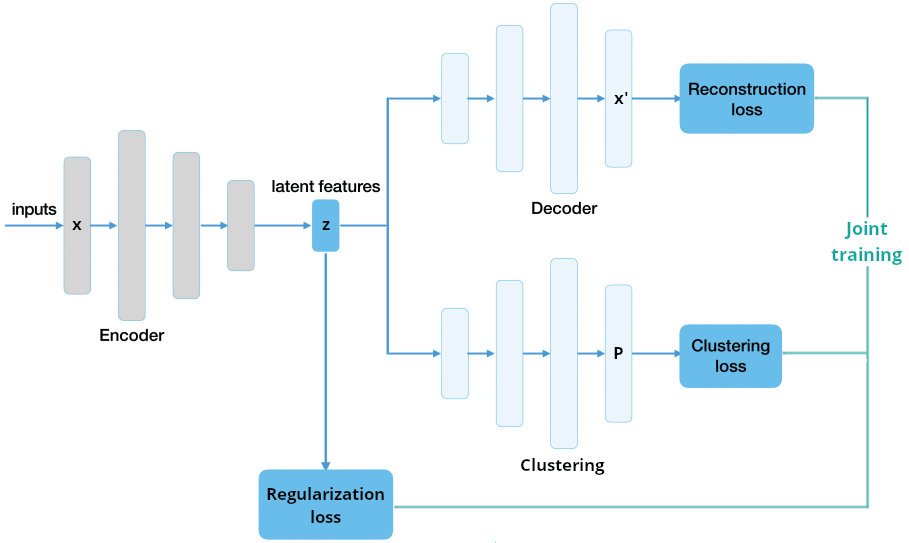
\includegraphics[width=\textwidth]{min2018_losses.png}
            \caption{
                Esquema de les funcions de cost
                aplicades durant l'entrenament
                d'un model de \textit{deep clustering}
                basat en arquitectura \gls{vae}.
                Font: adaptada de Min \textit{et. al.}, 2018 \citep{Min2018}
            }
            \label{fig:vae_losses}
        \end{figure}


    \subsection{Evaluation metrics}
    \label{s:metrics}

\todo{
    \begin{itemize}
        \item Llegir literatura
        \item Escollir mètodes
        \item Explicar mètodes seleccionats
    \end{itemize}}
\newpage

    \section{Software}
    \label{s:software}

        \paragraph{Eina per desenvolupar xarxes neuronals.}

            Per la realització d'aquest estudi es necessitarà desenvolupar models de xarxes neuronals complexos. Les eines més utilitzades actualment per treballar amb xarxes neuronals son TensorFlow, Keras i PyTorch \citep{Kaggle2021}.

            Keras \citep{Chollet2015} és una eina basada en TensorFlow \citep{Ghemawat2016} que es va desenvolupar per l'àmbit de la recerca. Permet definir i entrenar models de xarxes neuronals profunds de manera relativament senzilla, però alhora possibilita interactuar a més baix nivell amb TensorFlow per realitzar operacions més complexes \citep{Ketkar2021}.

            S'ha decidit treballar amb aquest eina donada la seva popularitat en l'àmbit de la recerca, i el fet que l'autor ja està familiaritzat a un nivell bàsic amb aquesta eina donat que s'ha utilitzat en l'assignatura M0.163 - Machine Learning del màster.

        \paragraph{Llenguatge de programació.}

            Les tècniques de \textit{clustering}, tant mitjançant mètodes de \textit{deep learning} com clàssics, podrien aplicar-se utilitzant una gran varietat de llenguatges de programació. En l'àmbit de la recerca són àmpliament utilitzats els llenguatges \textsf{R} \citep{RCoreTeam2017} y Python \citep{VanRossum2009} \citep{Kaggle2021}, donada la facilitat de compartir i replicar codi que aporta emmarcar-lo en llenguatge Markdown mitjançant documents R Markdown \citep{Xie2016} o llibretes Jupyter Notebook \citep{Kluyver2016}.

            Per realitzar els estudis de \textit{clustering} utilitzant tècniques clàssiques s'escull el llenguatge \textsf{R} i l'entorn de desenvolupament \textsf{R} Studio \citep{RStudioTeam2020}, donada la familiaritat adquirida amb aquest llenguatge i entorn en diverses assignatures del màster.

            Encara que existeix una llibreria que permet utilitzar Keras dins de l'entorn de \textsf{R}, el seu us és limitat donat que l'eina està desenvolupada en Python. En el seu llenguatge natiu és possible utilitzar Keras per realitzar tasques més complexes, com desenvolupar models més complexos i ajustar els mètodes d'entrenament o mesures del rendiment. S'escull per tant el llenguatge Python per realitzar els estudis de \textit{deep clustering}.

        \paragraph{Hardware i serveis de computació \textit{on-line}.}

            Encara que l'estudi amb mètodes clàssics utilitzant \textsf{R} es pot realitzar de manera local en un ordinador de sobretaula relativament modern, l'entrenament i execució dels models de \textit{deep learning} com els que s'utilitzaran en aquest estudi requereixen un hardware més potent del que es disposa. S'optarà per tant per l'ús de plataformes de computació \textit{on-line} àmpliament utilitzades tant per estudiants com en l'àmbit de la recerca: Google Colab\footnote{\url{https://research.google.com/colaboratory/faq.html}} i/o Paperspace Gradient\footnote{\url{https://docs.paperspace.com/gradient/}}.

            Com a valor afegir, la utilització d'aquests serveis facilitarà l'ús del software necessari, ja que posen a disposició un entorn Python amb gran varietat de llibreries preinstal·lades, com per exemple les necessàries per utilitzar Keras. Això elimina els possibles problemes o incompatibilitats que es podrien trobar al instal·lar tot el software necessari i facilita treballar amb les versions més recents.

            Ambdues plataformes ofereixen un model de subscripció gratuïta així com diferents plans de pagament. El model gratuït es considera insuficient en ambdós casos ja que no garanteix la disponibilitat de màquines virtuals en qualsevol moment, i això podria obstaculitzar el progrés del treball. El pla de pagament més econòmic d'ambdues plataformes té un preu similar i a priori es considera suficient per realitzar aquest estudi.

            Al comparar detalladament les característiques que ofereix cada servei, s'observa que Paperspace Gradient ofereix algunes característiques desitjables que no ofereix Google Colab: 15 GB d'emmagatzematge permanent, la opció de treballar amb una IDE completa de JupyterLab, i l'accés garantit a màquines amb característiques específiques. Per contra, cap pla de pagament de Google Colab garanteix la disponibilitat de màquines en qualsevol moment o les seves característiques.

            Per aquests motius, es decideix que es treballarà amb la plataforma Paperspace Gradient. S'estima que es necessitarà una subscripció durant els mesos de novembre i desembre, el que suposarà un cost econòmic de \$16.00 (equivalent a 16.44€ en el moment de la redacció d'aquest informe).

    \section{Més coses}
    \label{s:mes}

    Aquest TFM es divideix en dues parts ben diferenciades. A la primera part, emmarcada per l'objectiu 1.1 definit a la \cref{s:objectius}, es pretén consolidar una base sòlida de coneixements i habilitats específics que es posaran en pràctica a la segona part, que engloba els objectius 1.2 i 1.3.

    Es realitzarà una recerca bibliogràfica per tal de contextualitzar el problema a resoldre. Es caracteritzaran les tècniques de \textit{clustering} utilitzades en dades metabolòmiques i com s'utilitzen les tècniques de \textit{deep learning} en aquest camp.

    S'estudiarà amb profunditat l'arquitectura dels variational autoencoders i com es poden aplicar per realitzar tècniques \textit{clustering}. Finalment, s'estudiarà el funcionament de la llibreria Keras per desenvolupar xarxes neuronals. Per familiaritzar-se millor amb aquesta eina, es practicarà replicant exemples de codi ja desenvolupats. L'estudi es basarà en el manual \textit{Deep Learning with Python} \citep{Ketkar2021}.

    Per obtenir les dades metabolòmiques que s'utilitzaran per desenvolupar el model es contactarà amb un grup de treball de la Universitat de Barcelona associat amb el tutor d'aquest TFM.

    Per tal d'establir un marc de referència contra el que comparar el model que es desenvoluparà, es realitzarà un estudi de \textit{clustering} preliminar utilitzant algunes tècniques clàssiques consolidades.

    A continuació es durà a terme la part central del TFM: el desenvolupament d'un model de \textit{deep clustering} utilitzant una arquitectura de \textit{variational autoencoder}. Durant el desenvolupament es provaran diverses configuracions de xarxes neuronals, hiperparàmetres i mètodes d'entrenament per buscar una solució òptima. Un cop desenvolupat el model, es compararan els resultats obtinguts amb el marc de referencia.

    Finalment s'aplicarà el model sobre un conjunt de dades metabolòmiques procedents d'un estudi clínic i s'estudiarà la interpretabilitat del resultats. S'espera que el model tingui poder predictiu, és a dir que existeixi una relació entre els clústers generats i els grups reals definits a les dades.

    \paragraph{Conjunt de dades.}

        Els models de \textit{deep learning} requereixen una bona quantitat de dades per realitzar el seu entrenament. Aquestes dades es podrien obtenir d'algun repositori de bases de dades d'accés lliure, per exemple Gene Expression Omnibus de NCBI\footnote{\url{https://www.ncbi.nlm.nih.gov/gds}} o MetaboLights de EMBL-EBI\footnote{\url{https://www.ebi.ac.uk/metabolights/}}. No obstant, amb l'ànim de realitzar un estudi fresc es prefereix treballar amb dades no publicades, sempre que sigui possible.

        Es contactarà amb un grup de treball de la Universitat de Barcelona associat amb el tutor d'aquest TFM, que està realitzant un estudi relacionat amb dades metabolòmiques, per sol·licitar l'accés a les seves dades.

        En cas de no aconseguir-se per aquest mètode, s'intentarà contactar amb altres grups de treball relacionats amb dades òmiques per intentar aconseguir un conjunt dades adequada. Com a darrera opció, es cercarà una base de dades d'accés lliure que sigui adequada per realitzar aquest estudi.



\chapter{Resultats}
    %Detalleu en aquest apartat els resultats obtinguts utilitzant la metodologia descrita a l’apartat anterior.
    %Recull dels resultats del treball. Hauria d'haver-hi una correspondència amb la metodologia en el sentit que els resultats és el que s'obté després d'haver aplicat la metodologia.
    %Les figures han d'estar explicades i citades en el text, com la \ref{fig:my_label}, en la qual es mostra l'error en funció de la distància, en unitats arbitràries. A totes les gràfiques ha d'haver el títol dels eixos.
    %\begin{figure}[!htbp]
    %    \centering
    %    \includegraphics[width=7truecm]{Rplotmanh.png}
    %    \caption{Error en funcio de la distància en unitats arbitràries.}
    %    \label{fig:my_label}
    %\end{figure}

\chapter{Discussió}
    %Discussió dels resultats en el context del projecte. És en aquest apartat on cobren sentit i en el qual es responen les preguntes de recerca i es mostra com els resultats donen resposta als problemes plantejats.
    %Aquesta part pot ser que no apliqui segons el tipus de treball.

\chapter{Valoració econòmica}
    %En cas que correspongui, s'inclourà un apartat de ``Valoració econòmica del treball". Aquest apartat indicarà les despeses associades al desenvolupament i manteniment del treball, així com els beneficis econòmics obtinguts. Cal fer una anàlisi final sobre la viabilitat del producte.

\chapter{Conclusions i treballs futurs}

    \section{Conclusions}
        %Aquest capítol ha d'incloure:
        %\begin{itemize}
        %    \item Una descripció de les conclusions del treball:
        %    \begin{itemize}
        %        \item Un cop s’han obtingut els resultats quines conclusions s’extreu?
        %        \item Aquests resultats són els esperats? O han estat sorprenents? Per què?
        %    \end{itemize}
        %    \item Una reflexió crítica sobre l’assoliment dels objectius plantejats inicialment:
        %    \begin{itemize}
        %        \item Hem assolit tots els objectius? Si la resposta és negativa, per quin motiu?
        %    \end{itemize}
        %\end{itemize}


    \section{Línies de futur}
        %Les línies de treball futur que no s'han pogut explorar en aquest treball i han quedat pendents.

    \section{Seguiment de la planificació}
        %\begin{itemize}
        %    \item Una anàlisi crítica del seguiment de la planificació i metodologia al llarg del producte:
        %    \begin{itemize}
        %        \item S’ha seguit la planificació?
        %        \item La metodología prevista ha estat prou adequada?
        %        \item Ha calgut introduir canvis per garantir l’èxit del treball? Per què?
        %    \end{itemize}
        %    \item Dels impactes previstos a \ref{s:etic}, ètic-socials, de sostenibilitat i de diversitat, avaluaeu/esmenteu si s'han mitigat (si eren negatius) o si s'han aconseguit (si eren positius).
        %    \item Si han aparegut impactes no previstos a \ref{s:etic}, avaluar/esmentar com s'han mitigat (si eren negatius) o què han aportat (si eren positius).
        %\end{itemize}

\chapter{Glossari i abreviacions}
    %Definició dels termes i acrònims més rellevants utilitzats dins la Memòria.

    \section{Glossari}

    %Abreviacions:
    \printglossary[type=\acronymtype, title={Abreviacions}]

%\chapter{Bibliografia} %\bibliography{} ja afegeix el \chapter{} corresponent!
\bibliographystyle{ieeetr}
\bibliography{TFM, TFM-software}


\newpage
\appendix
%Llistat d’apartats que són massa extensos per incloure dins la memòria i tenen un caràcter autocontingut (per exemple, manuals d’usuari, manuals d’instal·lació, etc.)
%Depenent del tipus de treball, és possible que no calgui afegir cap annex.

%\chapter{Exemple d'annex}
%    \section{Annex 1}
%
%
%\chapter{Exemple d'annex}
%    \section{Annex B}


\end{document}
